%%%%%%%%%%%%%%%%%%%%%%%%%%%%%%%%%%%%%%%%%%%%%%%%%%%%%%%%%%%%%%%%%%%%%%%% 
%%%%%%%%%%%%%%%%%%%%%%%%%%%%%%%%%%%%%%%%%%%%%%%%%%%%%%%%%%%%%%%%%%%%%%%% 
\begin{frame}
  \frametitle{Performance portability}

  \begin{itemize}
  \item \textbf{Developing / maintaining} a \textcolor{red}{\textbf{separate}} implementation of an application for each \textbf{new hardware platform} (Intel KNL, Nvidia GPU, ARMv8, ...) is \textcolor{red}{\textbf{less and less realistic}}
  \item \textbf{Identical code} will never perform \textbf{optimally} on all platforms~\footnote{source: Matt Norman, \myhref{http://waccpd.org/wp-content/uploads/2016/04/WACCPD_2016_Norman.pdf}{WACCPD 2016}}
  \item Is it possible to have a \textcolor{blue}{\textbf{single set of source codes}} that can be compiled for different hardware targets ?
  \item Performance portability should be understood as a single source code base with
    \begin{itemize}
    \item \textcolor{darkgreen}{\textbf{good}} performance on different architectures
    \item a relatively \textcolor{darkgreen}{\textbf{small amount of effort}} required to tune app performance from one architecture to another.\\
      {\tiny source \myurl{http://www.nersc.gov/research-and-development/application-readiness-across-doe-labs}}
    \end{itemize}
  \item \textcolor{orange}{\textbf{High Developper / programmer productivity}}
    % \begin{itemize}
    % \item CPU vector length: 256 bits (8 \textit{vector threads})\\
    %   \textcolor{red}{Heavily cache-based}
    % \item KNL vector length: 512 bits  x  2 (16-32 \textit{vector threads})\\
    %   Moderately cache-based, some latency/bandwidth hiding
    % \item GPU vector length: 65 536 bit (2048 \textit{GPU vector threads})\\
    %   Less cache-based, heavy on latency/bandwidth hiding
    % \end{itemize}
  \end{itemize}

\end{frame}

%%%%%%%%%%%%%%%%%%%%%%%%%%%%%%%%%%%%%%%%%%%%%%%%%%%%%%%%%%%%%%%%%%%%%%%% 
%%%%%%%%%%%%%%%%%%%%%%%%%%%%%%%%%%%%%%%%%%%%%%%%%%%%%%%%%%%%%%%%%%%%%%%% 
\begin{frame}
  \frametitle{Performance portability issue : algorithmic patterns}

  \begin{itemize}
  \item Is it possible to have a single set of source codes that can be compiled for different hardware targets ?
  \item \textcolor{red}{\textbf{Low-level native language:}} OpenCL, CUDA, ...
  \item \textcolor{orange}{\textbf{Directive approach (code annotations)}} for multicore/GPU, ...: 
    \begin{itemize}
    \item \myhref{http://www.openmp.org/}{OpenMP} 4.5 (Clang, GNU, PGI, ...)
    \item \myhref{http://www.openacc.org/}{OpenACC} 2.5 (PGI, GNU, ...)
    \end{itemize}
  \item \textcolor{darkgreen}{\textbf{Other high-level library-based approaches}} (mostly c++-based, à la TBB):
    \begin{itemize}
    \item Some provide STL-like algorithmics patterns (e.g. \myhref{https://github.com/thrust/thrust}{Thrust} is CUDA-based with backends for other archs, \myhref{https://github.com/nsubtil/lift.git}{lift}, \myhref{https://github.com/arrayfire/arrayfire}{arrayFire} (numerical libraries, language wrappers, ...))
    \item \myhref{https://github.com/kokkos/kokkos}{Kokkos}, \myhref{https://github.com/LLNL/RAJA}{RAJA}, \myhref{https://github.com/agency-library/agency}{agency}, ...
    \item Cross-platform frameworks
      \begin{itemize}
      \item \myhref{http://charmplusplus.org/}{Chamm++}: message-driven execution, task and data migration, distributed load-balancing, ...
      \item \myhref{https://github.com/STEllAR-GROUP/hpx}{hpx} (heavy use of new c++ standards (11,14,17): \texttt{std::future, std::launch::async}, distributed parallelism, ...)
      \item \myhref{https://www.khronos.org/sycl}{SYCL} (Khronos Group \textit{standard}), one implementation by \myhref{https://www.codeplay.com/products/computesuite/computecpp}{CodePlay}, by \myhref{https://github.com/keryell/triSYCL}{Keryell/Xilinx}, ..., \myhref{https://github.com/KhronosGroup/SyclParallelSTL}{parallel STL}
      \end{itemize}
    \end{itemize}
  {\small \item \textcolor{darkblue}{\textbf{Use an embedded Domain Specific Language (DSL)}}
    \begin{itemize}
    \item \myhref{http://halide-lang.org/}{Halide} (for image processing),
    \item \myhref{http://www.nabla-lang.org/}{NABLA} (for HPC, developped at CEA, PDE mesh+particules apps)
    \end{itemize}}
  \end{itemize}

  {\small \myhref{https://www.khronos.org/assets/uploads/developers/library/2016-supercomputing/SC16-compareSYCL-Michael-Wong_Nov16.pdf}{SC16-compareSYCL-Michael-Wong\_Nov16.pdf}}
  
\end{frame}


%%%%%%%%%%%%%%%%%%%%%%%%%%%%%%%%%%%%%%%%%%%%%%%%%%%%%%%%%%%%%%%%%%%%%%%% 
%%%%%%%%%%%%%%%%%%%%%%%%%%%%%%%%%%%%%%%%%%%%%%%%%%%%%%%%%%%%%%%%%%%%%%%% 
\begin{frame}
  \frametitle{Performance portability issue : memory management}

  \begin{itemize}
  \item Right now \textbf{directives-based approaches} focus on algorithmic pattern, and less on memory layout (might change in the near future, at least in OpenMP).
  \item CPU and GPU for example require \textcolor{blue}{\textbf{different memory layout}} for \textcolor{darkgreen}{\textbf{maximun performance:}}
    \begin{itemize}
    \item vectorization on CPU
    \item memory coalescence on GPU
    \end{itemize}
  \item Some libraries like \myhref{https://github.com/kokkos/kokkos}{Kokkos} promote \textcolor{blue}{\textbf{memory layout}} as a \textcolor{darkgreen}{\textbf{major concern}}
  \end{itemize}

  \begin{center}
    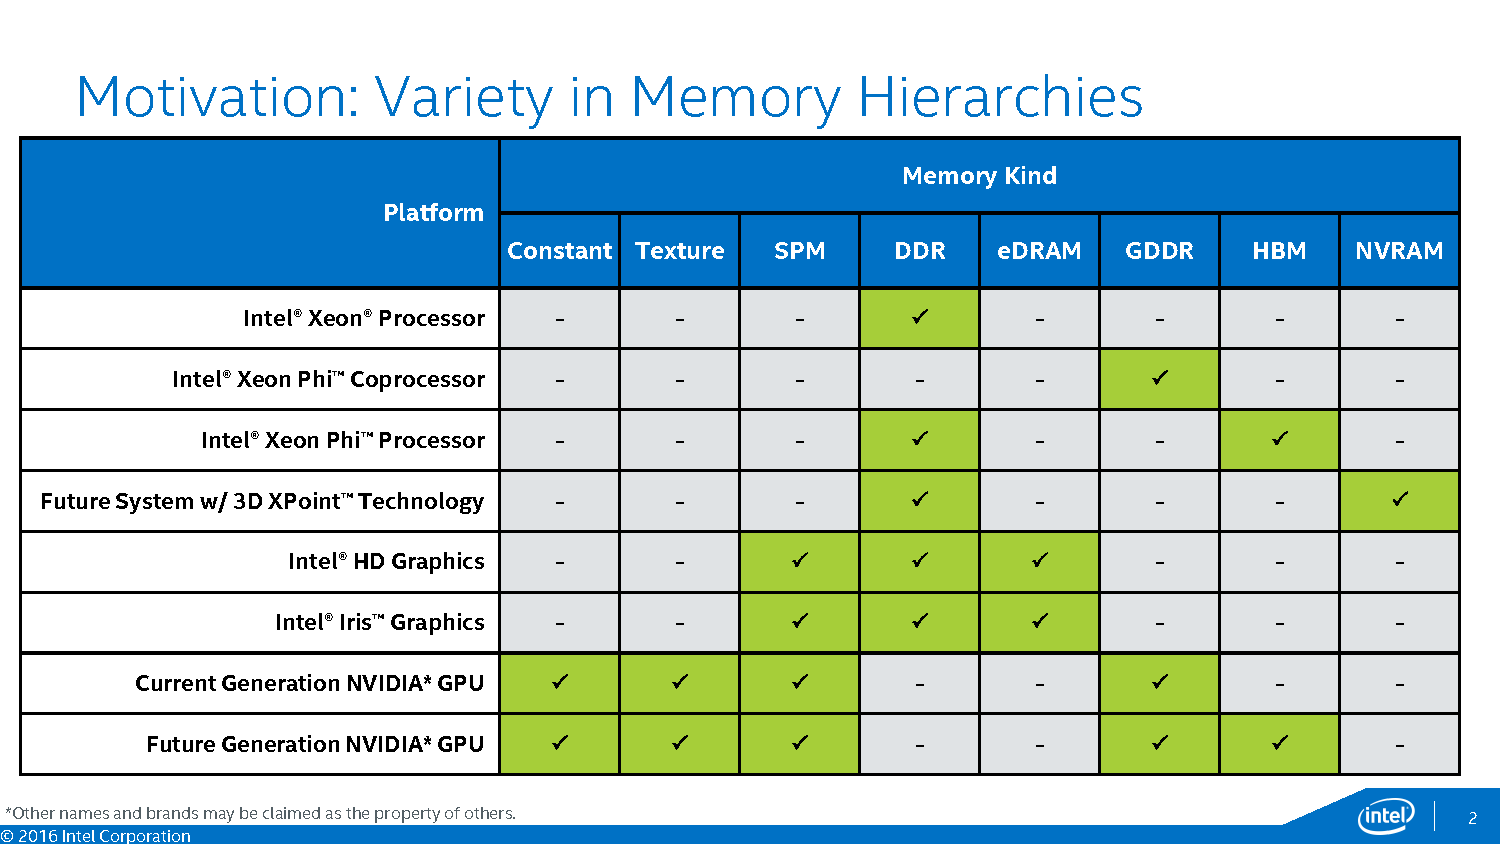
\includegraphics[width=6cm]{doc/openmp/omp_memory}
  \end{center}


\end{frame}

